\documentclass{article}
\usepackage[utf8]{inputenc}
\usepackage{amsmath}
\usepackage{graphicx}

\title{Reporte de actividades semestre Marzo a Agosto 2021}
\author{Julio César Pérez Pedraza}
\date{Septiembre de 2021}

\begin{document}

\maketitle

\section{Introducción}
En el primer semestre de doctorado se estudió la teoría en que se basará el trabajo de investigación. En particular, se aprendió el método de Lattice Boltzmann (LBM), el cual es un método a escala mezoscópica y desarrollado a partir de la teoría cinética, utilizado ampliamente para la simulación de sistemas hidrodinámicos. Además, se aprendió a utilizar el lenguaje de programación "C" para la implementación de cálculos numéricos usando el RRLBM. Posteriormente, durante el segundo semestre, se estudió el método de Lattice Boltzmann Relativista (RLBM) en 3 dimensiones, el cual describe la hidrodinámica de fluidos que se mueven a velocidades cercanas a la velocidad de la luz (como resluta ser para el grafeno). A la par, se implementaron algunos programas de LBM para el caso clásico a modo de práctica, tales como los flujos de Poiseuille y el vórtice de Taylor-Green.\\

Durante el semestre que apenas concluyó (tercer semestre), de acuerdo al plan de trabajo estipulado, se trabajó en la implementación de programas para el caso del RLBM. En primera instancia, se aplicó dicho método en 3 dimensiones (reducidas a una dimensión) para el problema de Riemann en materia gluónica viscosa, el cuál nos sirvió para corroborar la aplicabilidad de dicho modelo. Se prosiguió aplicando el RLBM a sistemas de grafeno. Para ello, primero se adaptó el modelo al caso de dos dimensiones y posteriormente se implementó el método para varios sistemas de grafeno, de donde se calcularon algunas propiedades de transporte en el material en cada caso.\\

A continuación se da un breve resumen del trabajo desarrollado en este semestre. Se comienza con la implementación del RLBM aplicada al problema de Riemann en el plasma quark-gluón. Enseguida, se muestran las modificaciones que sufre el RLBM al adaptarlo al caso 2D (de grafeno). Posteriormente, se muestran resultados de implementaciones del modelo 2D para algunos sistemas de grafeno. 

\section{El problema de Riemann en el plasma quark-gluón usando el RLBM}

El problema de Riemann consiste en un sistema cuya configuración inicial consiste de dos regiones divididas por una membrana, las cuales se encuentran en equilibrio termodinámico, pero en cada región se tienen valores distintos para la presión. En el caso de la materia gluónica viscosa, consideramos un sistema unidimensional con ecuación de estado ultrarrelativista para la energía $\epsilon = 3P$, y con la densidad de energía y la densidad de número de partículas relacionadas por $\epsilon=3nT$, donde $T$ es la termperatura del sistema. Se localiza la membrana en $z=0$ y las presiones para las regiones $z<0$ y $z>0$ están dadas por $P_0$ y $P_1$ respectivamente. Al tiempo $t=0$ la membrana es retirada y el fluido se comienza a expandir.\\

Para implementar dicho sistema, basándonos en\footnote{M. Mendoza, B. M. Boghosian, H. J. Herrmann, and S. Succi, \textit{Derivation of the lattice Boltzmann Model for relativistic hydrodynamics}, Phys. Rev D \textbf{82}, 105008 (2010).}, usamos el RLBM en una dimensión (una red de $1\times1\times800$), donde para este caso la cuadri-velocidad está dada por $u^{\mu}=\gamma(1,0,0,\beta)^{\mu}$. La velocidad de red está dada por $c_l=1.0$. El tamaño de celda y de paso temporal se escogen como $\delta x = 0.008 fm$ y $\delta t = 0.008 fm/c$, respectivamente. Se calcula la viscosidad como $\eta=\frac{4}{9}\gamma \epsilon(\tau-1/2) $ y la densidad de entropía como $s= n(4-ln\lambda)$, con $\lambda=\frac{n}{n^{eq}}$ la fugacidad del gluón. La densidad de partículas en equilibrio está dada por $n^{eq}=\frac{d_G T^3}{\pi^2}$, donde $d_G=16$ para gluones. Se fijan las presiones $P_0=5.43 GeVfm^{-3}$ y $P_1=2.22 GeVfm^{-3}$ correspondientes en unidades numéricas a $P_0=7.9433\times 10^{-6}$ y $P_0=3.2567\times 10^{-6}$, respectivamente. Además, se fija la temperatura inicial del sistema a $T_0=350MeV$ correspondiente a $T_0=0.0287$ en unidades numéricas. Las condiciones de frontera en los extremos se toman libres.\\

En la figura 1 se observa el perfil de la onda de choque luego de una evolución temporal de 500 pasos (velocidad y presión en cada región del sistema). Se observa una gran concordancia con las curvas obtenidas por otros métodos, por lo que se concluye que el modelo trabaja bien para estos sistemas relativistas.

\begin{figure}[th!]
   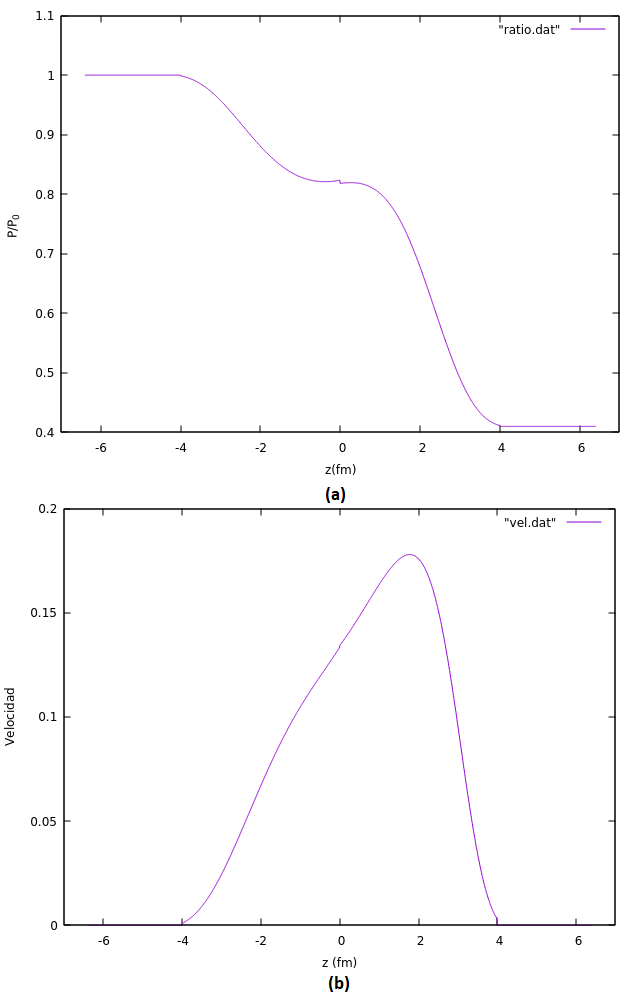
\includegraphics[width=0.89\columnwidth]{riemann.png}
   \caption{Problema de Riemann para el quark-gluon plasma usando el RLBM en 3D. (a)Presión y (b)velocidad del sistema despues de una evolución temporal de $800 fm/c$ (500 pasos).}
   % \label{fig:red}
\end{figure}

\section{Adaptación del RLBM al caso 2D (grafeno)}
\subsection{Caso 3D}
En el reporte anterior se desarrolló la ecuación de Boltzmann en 3 dimensiones a partir del tensor de energía momento
\begin{equation}
    T^{\mu\nu} = P \eta^{\mu\nu} + (\epsilon + P) u^\mu u^\nu+ \pi^{\mu\nu},
\end{equation}
y del cuadri-vector de flujo de partículas (cuadri-flujo)
\begin{equation}
    N^\mu = n \gamma (1, \vec{\beta})^\mu, 
\end{equation}
donde en la primera ecuación $\epsilon$ es la densidad de energía, $P$ la presión hidrostática, y $\pi^{\mu\nu}$ la componente disipativa del tensor de energía-momento, mientras que en la segunda ecuación $n$ denota el número de partículas por unidad de volumen. Además, se define el cuadri-vector de velocidad (cuadri-velocidad) como 
\begin{equation}
    u^\mu = ( \gamma, \gamma \vec{\beta}),
\end{equation}
donde $\vec{\beta}= \vec{u}/c$ es la velocidad del fluido en unidades de la velocidad de la luz, y $\gamma =1/ \sqrt{1-|\vec{\beta}|^2}$ es el factor de Lorentz. El tensor $\eta^{\mu\nu}$ denota la métrica de Minkowski. \\

 Aplicando estas definiciones, se llega a condiciones de conservación de energía-momento y de número de partículas ("fonones" y "fluones"). También, utilizando la aproximación para el operador de colisión dado por el modelo de Marle modificado, además del set de velocidades dicreto $D3Q19$, donde la velocidad máxima de movimiento de las partículas es $\sqrt{2}c_l$, con $c_l = \frac{\delta x}{\delta t}$, y en donde las unidades de velocidad son reescaladas de modo que $c\sim 1$, se obtiene que ambas ecuaciones de lattice Boltzmann tienen la misma cara que para el caso clásico
\begin{equation}
    f_i(\vec{x} + \vec{c}_i\delta t, t + \delta t) -f_i (\vec{x}, t) = - \frac{\delta t}{\tau} (f_i - f_i^{eq}),
\end{equation}
y
\begin{equation}
    g_i(\vec{x} + \vec{c}_i\delta t, t + \delta t) -g_i (\vec{x}, t) = - \frac{\delta t}{\tau} (g_i - g_i^{eq}),
\end{equation}
con $\tau$ representando el tiempo de relajación realista del sistema.\\

Las variables hidrodinámicas se calcula usando las siguientes restricciones macroscópicas
\begin{subequations}
\begin{equation}
    n\gamma = \sum_{i=0}^{18} f_i, 
\end{equation}
\begin{equation}
    (\epsilon+P) \gamma^2-P = \sum_{i=0}^{18} g_i, 
\end{equation}
\begin{equation}
    (\epsilon+P) \gamma^2 \vec{u} = \sum_{i=0}^{18} g_i \vec{c}_i. 
\end{equation}
\end{subequations}
Se tienen cinco ecuaciones y seis incógnitas ($n$, $\epsilon$, $P$ y $\vec{u}$), por lo que se ciera el sistema escogiendo una ecuación de estado, que este caso tomamos como $\epsilon= 3P$ (caso 3D).\\
    
Para calcular las funciones de distribución de equilibrio que recuperan las ecuaciones de fluidos relativistas se usa el procedimiento de "moment-matching" entre las funciones de equilibrio y reglas de conservación (6a-c)
\begin{subequations}
\begin{equation}
    f_i^{eq} = w_i [A + \vec{c}_i \cdot \vec{B}], \ \ for \ \ i\geq 0, 
\end{equation}
\begin{equation}
    g_i^{eq} = w_i [C + \vec{c}_i \cdot \vec{D} + E:(\vec{c}_i \vec{c}_i -\alpha I], \ \ for \ \ i > 0, 
\end{equation}
\begin{equation}
g_0^{eq} = w_0 [F], 
\end{equation}
 \end{subequations}
 donde $\alpha$, $A$, $\vec{B}$, $C$, $\vec{D}$, $\overleftrightarrow{E}$ y $F$ son parámetros de Lagrange. Usando los pesos definidos por $w_0=1/3$, $w_i=1/18$ para velocidades con magnitud $|\vec{c}_i|=c_l$ y $w_i = 1/36$ para velocidades con $|\vec{c}_i|=\sqrt{2}c_l$, se obtuvieron los valores para los parámetros de Lagrange: $A=n\gamma$, $\vec{B}= \frac{
 3}{c_l^2}\gamma n \vec{u}$, $\alpha= \frac{c_l^2}{3}$, $C=\frac{3P}{c_l^2}$, $\vec{D}= \frac{3}{c_l^2}(\epsilon+P) \gamma^2 \vec{u}$, $E_{ab}=\frac{9}{2c_l^4}(\epsilon+P) \gamma^2 u_a u_b$ y $F= (\epsilon+P) \gamma^2\left[ 3- 3\frac{(2+c_l^2)P}{c_l^2(\epsilon+P)\gamma^2}- \frac{3}{2c_l^2} (\epsilon+P)\gamma^2|\vec{u}|^2 \right].$ Por lo tanto, se llega a las funciones de distribución de equilibrio que recuperan las ecuaciones de fluidos relativistas en el límite continuo dadas por
   \begin{equation}
     f_i^{eq} = w_i n\gamma\left[ 1+3 \frac{(\vec{c}_i\cdot \vec{u})}{c_l^2} \right], 
 \end{equation}
 para $i\geq 0$, 
 \begin{equation}
     g_i^{eq} = w_i\epsilon\gamma^2\left[ \frac{1}{c_l^2\gamma^2}+4 \frac{(\vec{c}_i\cdot \vec{u})}{c_l^2}+ 6 \frac{(\vec{c}_i\cdot \vec{u})^2}{c_l^4}-2\frac{|\vec{u}|^2}{c_l^2} \right], 
 \end{equation}
  para $i> 0$, y
   \begin{equation}
     g_0^{eq} = w_0\epsilon\gamma^2\left[4- \frac{2+c_l^2}{c_l^2\gamma^2}-2\frac{|\vec{u}|^2}{c_l^2} \right], 
 \end{equation}
 para $i=0$, donde se ha hecho la elección de la ecuación de estado $\epsilon=3P$.\\
 
 La viscosidad cortante se calcula como $\eta = \frac{4}{9} \gamma \epsilon (\tau-\delta t /2) c_l^2$. Además, es importante notar que este esquema relativista recupera suavemente el límite no-relativista simplemente haciendo $\beta \rightarrow 0$.

\subsection{Caso $2D$}
Para el caso $2D$ se deben tomar algunas consideraciones que hacen el cálculo diferente al caso $3D$. En primer lugar, la tercera componente espacial tanto del cuadri-vector de velocidad y del cuadri-flujo de partículas (Ecs. (2) y (3) ) se hace cero, llevándonos a ecuaciones de conservación de la energía y del numero de partículas en dos dimensiones.\\

Adicionalmente, la ecuación de estado que se había usado en el caso $3D$, $\epsilon =3P$ (límite ultrarrelativista), ahora cambia a $\epsilon =2P$.\\

También, ahora debe usarse un set de velocidades discreto en $2D$. En este caso trabajamos con el set $D2Q9$, por lo que, al realizar el "moment-matching" entre las funciones de equilibrio y reglas de conservación (Ecs. (6a-c)) las sumatorias solo van a correr hasta $8$. Además, los pesos para este set cambian con respecto al anterior, tomando ahora los valores $w_0=4/9$, $w_i=1/9$ para velocidades con magnitud $|\vec{c}_i|=c_l$ y $w_i = 1/36$ para velocidades con $|\vec{c}_i|=\sqrt{2}c_l$.\\

Siguiendo con el procedimiento de "moment-matching" con estas nuevas condiciones, se obtienen los mismos valores para los parámetros de Lagrange $A$, $\vec{B}$, $\alpha$, $C$, $\vec{D}$, $E_{ab}$, pero el parámetro $F$ ahora está dado por $F= (\epsilon+P) \gamma^2\left[ \frac{9}{4}- \frac{3}{4}\frac{(5+3c_l^2)P}{c_l^2(\epsilon+P)\gamma^2}- \frac{3}{2c_l^2} |\vec{u}|^2 \right].$ Por lo tanto, se llega a las funciones de distribución de equilibrio para el caso $2D$:
  \begin{equation}
     f_i^{eq} = w_i n\gamma\left[ 1+3 \frac{(\vec{c}_i\cdot \vec{u})}{c_l^2} \right], 
 \end{equation}
 para $i\geq 0$, 
 \begin{equation}
     g_i^{eq} = w_i(\epsilon+P)\gamma^2\left[ \frac{3P}{c_l^2(\epsilon+P)\gamma^2}+3 \frac{(\vec{c}_i\cdot \vec{u})}{c_l^2}+ \frac{9}{2} \frac{(\vec{c}_i\cdot \vec{u})^2}{c_l^4}-\frac{3}{2}\frac{|\vec{u}|^2}{c_l^2} \right], 
 \end{equation}
  para $i> 0$, y
   \begin{equation}
     g_0^{eq} = w_0(\epsilon+P) \gamma^2\left[ \frac{9}{4}- \frac{3}{4}\frac{(5+3c_l^2)P}{c_l^2(\epsilon+P)\gamma^2}- \frac{3}{2c_l^2} |\vec{u}|^2 \right], 
 \end{equation}
 para partículas en reposo. Además, para la ecuación de estado $\epsilon=2P$, estas ecuaciones se simplifican a 
   \begin{equation}
     f_i^{eq} = w_i n\gamma\left[ 1+3 \frac{(\vec{c}_i\cdot \vec{u})}{c_l^2} \right], 
 \end{equation}
 para $i\geq 0$, 
 \begin{equation}
     g_i^{eq} = w_i\epsilon\gamma^2\left[ \frac{3}{2c_l^2\gamma^2}+\frac{9}{2} \frac{(\vec{c}_i\cdot \vec{u})}{c_l^2}+ \frac{27}{4} \frac{(\vec{c}_i\cdot \vec{u})^2}{c_l^4}-\frac{9}{4}\frac{|\vec{u}|^2}{c_l^2} \right], 
 \end{equation}
  para $i> 0$, y
   \begin{equation}
     g_0^{eq} = w_0\epsilon\gamma^2\left[\frac{27}{8}-\frac{3}{8} \frac{(5+3c_l^2)}{c_l^2\gamma^2}-\frac{9}{4}\frac{|\vec{u}|^2}{c_l^2} \right], 
 \end{equation}
 para $i=0$. La viscosidad cortante para este caso es $\eta = \frac{1}{2} \gamma \epsilon (\tau-\delta t /2) c_l^2$. 
 
 \section{Implementación del RLBM en $2D$ para algunos sistemas de grafeno}
 Una vez que se obtuvieron las expresiones correctas para el RLBM en dos dimensiones, se prosiguió a aplicar el método a algunos sistemas de grafeno. En primer lugar, para ver si el modelo funcionaba (no explotaba), se implementó el modelo para el flujo de electrones en grafeno pristino (sin impurezas ni deformaciones). Posteriormente, con el propósito de medir la conductividad eléctrica y la fuerza de arrastre ("drag force") en el sistema, se procedió a insertar impurezas circulares (cilíndricas) en el sistema de grafeno pristino. Se estudiaron varias configuraciones de impurezas: una sola impureza, dos o más impurezas en linea con el mismo o diferente tamaño, y el caso más general, varias impurezas con posiciones y tamaños aleatoriamente elegidos. También, se implementó en el código una función que calcula la transformada rápida de Fourier (FFT) para encontrar las frecuencias naturales de oscilación de ambas cantidades mencionadas. Para cada caso se obtienen cálculos de la conductividad eléctrica y de la fuerza de arrastre con sus respectivos diagramas de la FFT. Además, si se eligen los parámetros adecuados de modo que $Re\approx 100$ y se deja evolucionar el sistema el suficiente tiempo, se obtienen patrones de turbulencia en la muestra. Esto se muestra a continuación para el caso de una impureza, el cual muestra un patrón muy similar al del caso de la "calle de vórtices de von Kármán".\\
 
 En todos los sistemas que se muestran a continuación, se ha utilizado el set de velocidades $D2Q9$ con sus respectivos pesos. Además, se han utilizado condiciones de frontera periódicas en los extremos inferior y superior. Para el extremo de la derecha (outlet) se tiene una condición de frontera libre, en donde el valor de las funciones de distribución se extrapolan de los sitios anteriores. Para los sitios en la frontera de la izquierda (inlet), el valor de las funciones de distribución se toman iguales al valor de la función de equilibrio con condiciones iniciales. El valor inicial de la densidad de energía se fija como $\epsilon = 0.75$; la densidad de número de cargas, $n=1.0$; la velocidad inicial se toma como $\textbf{u}=(0.002, 0)$. 
 
 \subsection{Grafeno pristino}
 Para el caso del grafeno pristino no hay mucho qué decir. El sistema rápidamente se estabiliza con una velocidad en la dirección $x$ igual a la velocidad inicial (Fig. 1). Lo importante para nosotros es que el modelo RLBM no explota para tiempos grandes.
 
\begin{figure}[th!]
   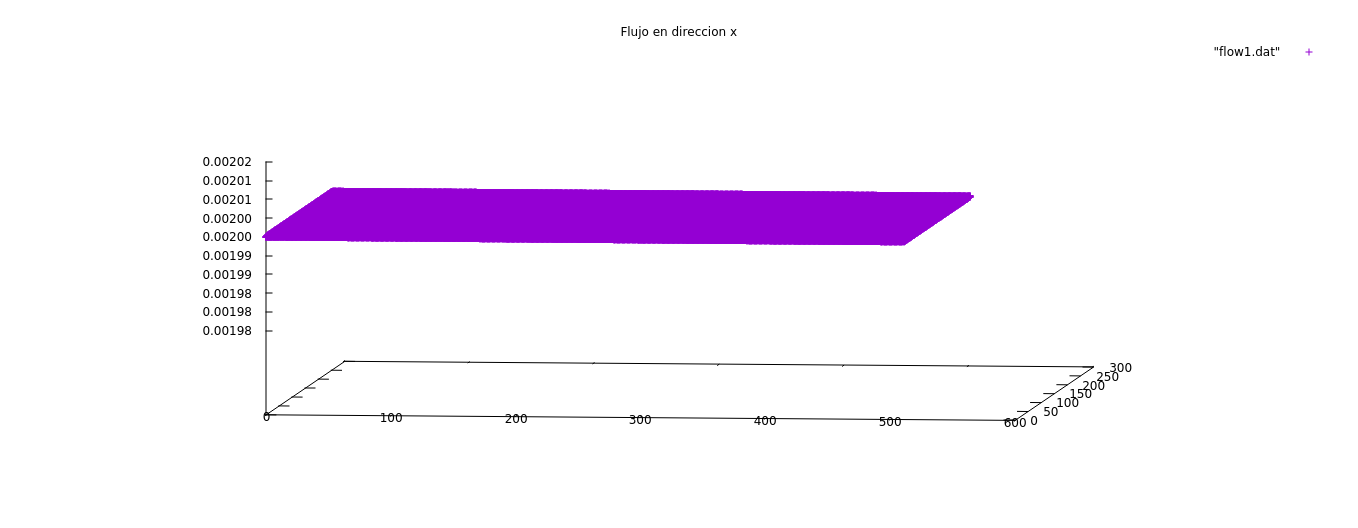
\includegraphics[width=1.16\columnwidth]{pristino.png}
   \caption{Flujo electronico en la dirección $x$ para el grafeno pristino.}
   % \label{fig:red}
\end{figure}
 
 
 \subsection{Una impureza}
 Cuando insertamos impurezas al sistema, estamos desestabilizando el flujo de electrones, por lo que se espera un cambio en la conductividad eléctrica. Para simular el sistema con impurezas se utiliza condiciones de frontera de "bounce back" (BB) en su superficie, esto es, se considera que cada población que tiene como destino un sitio frontera de la impureza regresa al sitio de donde proviene pero con la velocidad en dirección opuesta.\\
 
 En la figura 2 se observa la evolución temporal del flujo de electrones en la dirección $x$ para el sistema con una impureza circular de radio $r=25$ para $20,000$, $100,000$ y $4,000,000$ de pasos temporales. Además se toma un tiempo de relajación $\tau=0.503$, por lo que con esta elección de parámetros se obtiene un número de Reynolds, $Re=100$. Se observa cómo para estas condiciones específicas y tiempos suficientemente grandes se comienzan a formar patrones de turbulencia similares a la "calle de vórtices de von Kármán".\\
 
 \begin{figure}[th!]
   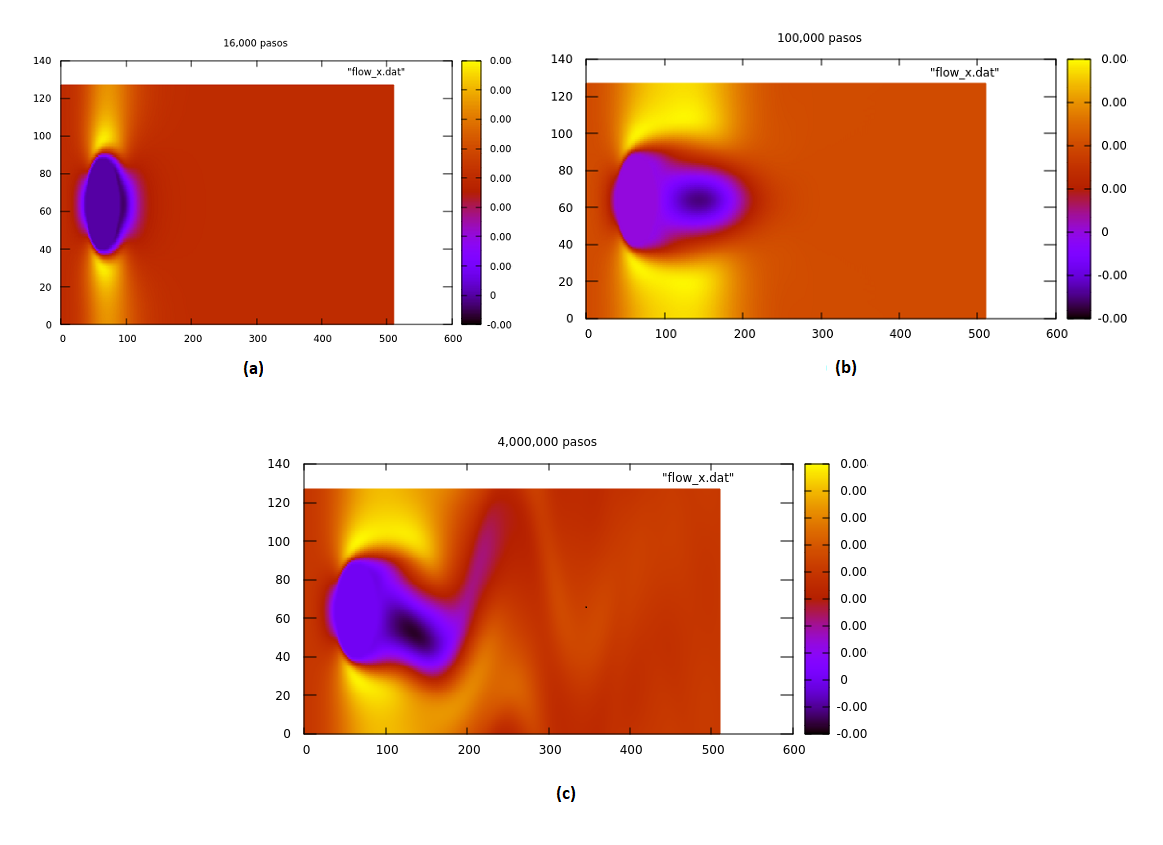
\includegraphics[width=1.1\columnwidth]{karrman.png}
   \caption{Mapa de calor sobre la evolución temporal del flujo de portadores de carga en la dirección $x$ en una red de grafeno con una impurezas de radio $r=25$. (a) 16,000 pasos. (b) 100,000 pasos. (c)4,000,000 pasos. }
   % \label{fig:red}
\end{figure}
 
 En las figuras 3 y 4 se observan los cálculos de la corriente eléctrica en un punto posterior a la impureza con respecto al paso temporal, y la fuerza de arrastre sobre la impureza, respectivamente. En ambos casos se muestra la FFT de las señales temporales.

\begin{figure}[th!]
   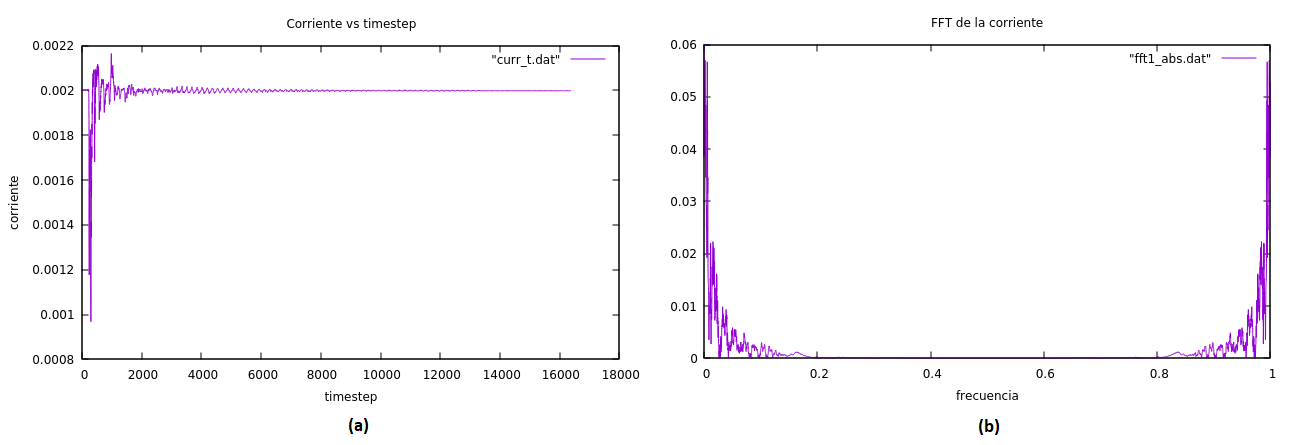
\includegraphics[width=1.1\columnwidth]{corriente_1obs.png}
   \caption{(a) Corriente eléctrica vs paso temporal para una red de grafeno con una impureza de radio $r=25$ en la posición $(64, 64)$. (b) FFT de la señal temporal de la corriente eléctrica.}
   % \label{fig:red}
\end{figure}

\begin{figure}[th!]
   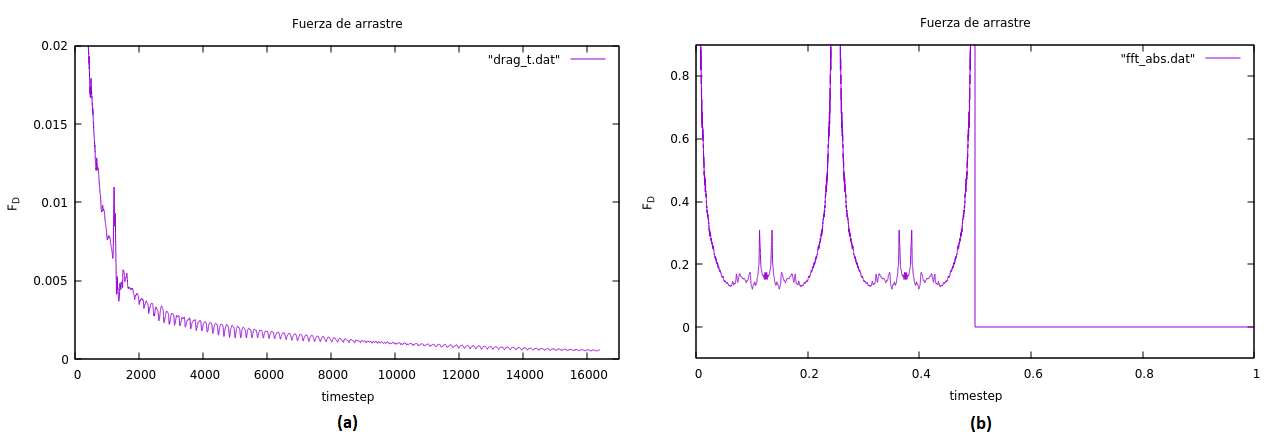
\includegraphics[width=1.1\columnwidth]{F_D_1obj.png}   \caption{(a) Fuerza de arrastre vs paso temporal para una red de grafeno con una impureza de radio $r=25$ en la posición $(64, 64)$. (b) FFT de la señal temporal de la fuerza de arrastre.}
   % \label{fig:red}
\end{figure}
 
 \subsection{Impurezas con posiciones y tamaños aleatorios}
 Para este caso se implementó una función que designa posiciones y tamaños de 5 impurezas de manera aleatoria (se puede implementar para un número arbitrario de impurezas). En la figura 5 se observa el flujo de electrones en la dirección $x$ para $16,000$ pasos temporales. 
\begin{figure}[th!]
   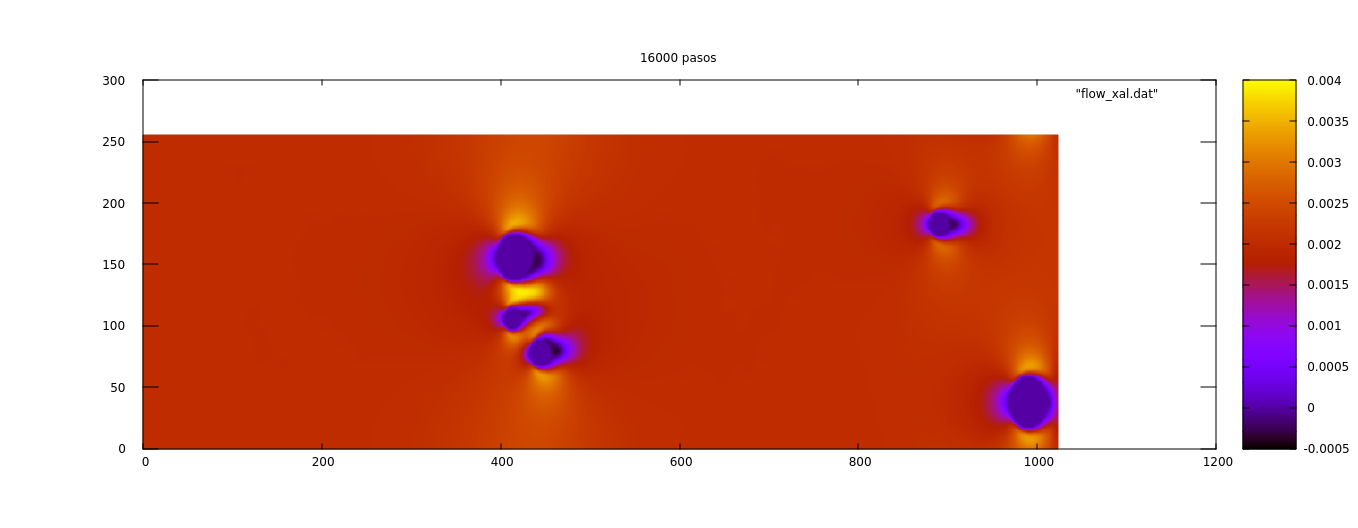
\includegraphics[width=1.0\columnwidth]{aleat.png}   \caption{Mapa de calor del flujo de portadores de carga en la dirección $x$ en una red de grafeno con cinco impurezas con radios y posiciones elegidas de manera aleatoria.}
   % \label{fig:red}
\end{figure}
 
  En las figuras 6 y 7 se observan los cálculos de la corriente eléctrica en un punto posterior a la zona com impurezas con respecto al paso temporal, y la fuerza de arrastre sobre la impureza, respectivamente. En ambos casos se muestra la FFT de las señales temporales.
  \begin{figure}[th!]
   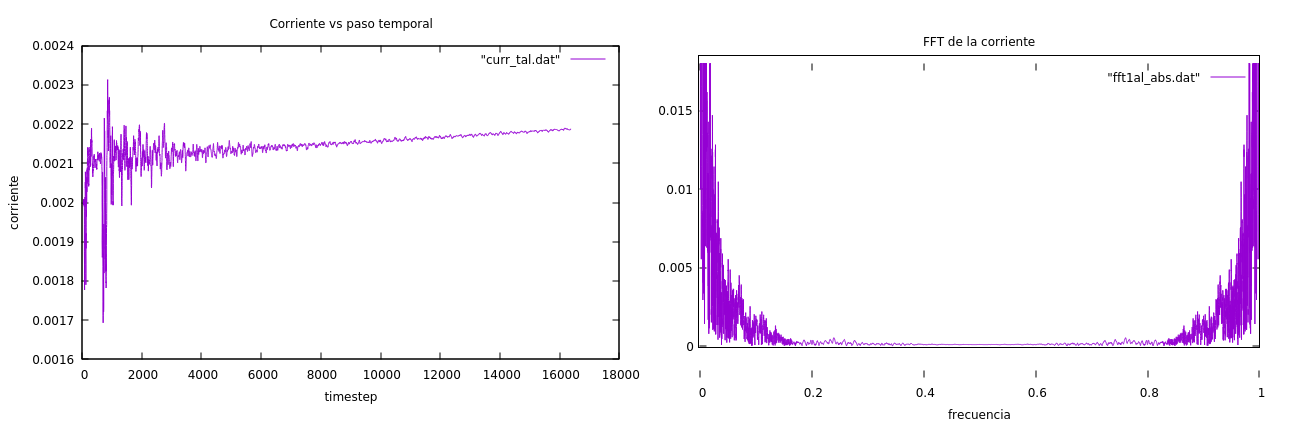
\includegraphics[width=1.1\columnwidth]{corr_aleat.png}   \caption{(a) Corriente eléctrica vs paso temporal para una red de grafeno con cinco impurezas con radios y posiciones elegidas de manera aleatoria.. (b) FFT de la señal temporal de la corriente eléctrica.}
   % \label{fig:red}
\end{figure}
\begin{figure}[th!]
   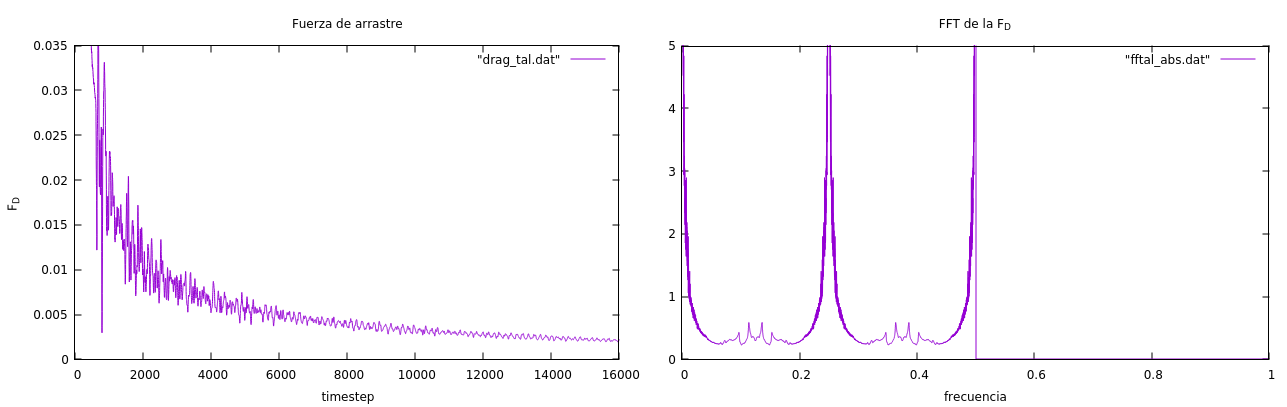
\includegraphics[width=1.1\columnwidth]{F_Dal.png}   \caption{(a) Fuerza de arrastre vs paso temporal para una red de grafeno con cinco impurezas con radios y posiciones elegidas de manera aleatoria.. (b) FFT de la señal temporal de la fuerza de arrastre.}
   % \label{fig:red}
\end{figure}
 
 \section{Trabajo en proceso y a futuro}
Como tenemos pretendido en el plan de trabajo de doctorado, comenzaremos con el estudio de redes neuronales (NN) en la plataforma de TensorFlow, para su aplicación en clasificación de sistemas de grafeno en un futuro. La idea principal es ser capaces de que la red nos diga qué configuración de grafeno con impurezas nos generaría algún perfil de corriente o de fuerza de arrastre (o alguna otra propiedad de transporte). Además, veremos si es posible aplicar campos externos a las simulaciones, para así tener un espectro más amplio. Adicionalmente, se está trabajando en aspectos teóricos de grafeno y la ecuación de Dirac.

\end{document}
